\documentclass{beamer}
\usepackage[utf8]{inputenc}
\usepackage{amsmath}
\usepackage{graphicx}

\usetheme{AnnArbor}
\usecolortheme{spruce}

\setbeamertemplate{itemize items}[default]
\setbeamertemplate{enumerate items}[default]

% define a darker brown
\definecolor{uwbrown}{HTML}{662200}
% apply dark brown to the item bullet points
\setbeamercolor{item}{fg=uwbrown}

\title[Física Moderna]{Física Moderna}
\subtitle{Ingeniería en Nanotecnología}
\author{Dr. Rubén Velázquez Hernández}
\institute[UTEQ]{Universidad Tecnológica de Querétaro}
\date{Cuatrimestre Mayo - Agosto 2025}
\logo{
\includegraphics[width=2cm]{../Imagenes/Logo_uteq}} % Ajusta la ruta 

\makeatletter
\setbeamertemplate{footline}
{
	\leavevmode%
	\hbox{%
		\begin{beamercolorbox}[wd=.25\paperwidth,ht=2.25ex,dp=1ex,center]{author in head/foot}%
			\usebeamerfont{author in head/foot}\insertshortauthor
		\end{beamercolorbox}%
		\begin{beamercolorbox}[wd=.55\paperwidth,ht=2.25ex,dp=1ex,center]{title in head/foot}%
			\usebeamerfont{title in head/foot}\insertshorttitle
		\end{beamercolorbox}%
		\begin{beamercolorbox}[wd=.2\paperwidth,ht=2.25ex,dp=1ex,right]{section in head/foot}%
			\usebeamerfont{section in head/foot}\insertframenumber{} / \inserttotalframenumber\hspace*{2ex}
	\end{beamercolorbox}}%
	\vskip0pt%
}
\makeatother

\begin{document}

\frame{\titlepage}

\begin{frame}
    \frametitle{BIENVENIDA}
    \begin{itemize}
        \item \textbf{Asignatura:} Física Moderna
        \item \textbf{Carrera:} Ingeniería en Nanotecnología
        \item \textbf{Modalidad:} Presencial asistida por tecnología
        \item \textbf{Período:} Mayo - Agosto 2025
        \item \textbf{Duración:} 60 horas totales (26 sesiones de 2 horas)
        \item \textbf{Plataforma:} Google Classroom
    \end{itemize}
\end{frame}

\begin{frame}[plain]
	\frametitle{¿Qué sucede a nivel cuántico?}
	\begin{figure}
		\centering
		
\includegraphics[width=.8\linewidth]{../Imagenes/AtomoR.jpg}
		%\caption{The caption of the figure.}
	\end{figure}	
\textit{\begin{flushright}
		"Si crees que entiendes la mecánica cuántica... es que no la entiendes." Richard Feynman
\end{flushright}}
	%% TODO: You can add the note here
	\note{}	
\end{frame}
	
\begin{frame}
    \frametitle{Objetivos del Curso}
   \begin{block}{Objetivo HA}
   		El alumno describirá el comportamiento de los materiales nanoestructurados con base en los conceptos, teorías y principios de física moderna para determinar sus características y propiedades.
   \end{block}
   \begin{block}{Objetivo General} 
   		 El alumno describirá los fenómenos fundamentales de la física moderna y aplicará sus principios (cuantización, dualidad, ecuación de Schrödinger) para comprender el comportamiento cuántico de la materia a nivel atómico y subatómico.
   		 
   		 Utilizará herramientas computacionales y de inteligencia artificial como apoyo para determinar las características y propiedades de materiales nanoestructurados.
    \end{block}
\end{frame}

\begin{frame}
    \frametitle{Competencia a Desarrollar}
   
   Fundamentar el diseño de procesos de producción de materiales nano-estructurados mediante la aplicación de los principios y modelos de la física moderna, para determinar sus características, propiedades y potenciales aplicaciones que contribuyan a la innovación tecnológica.
   
\end{frame}

\begin{frame}
    \frametitle{Unidades Temáticas}
    En Hoja de Asignatura
    \begin{enumerate}
    	\item Teoría básica del electromagnetismo  
    	\item Modelo nuclear del átomo 
    	\item Dualidad onda-partícula
    	\item Solución de la ecuación de Schrödinger
    \end{enumerate}
    
\end{frame}
\begin{frame}[plain]
	\frametitle{Mapa Curso}
	\begin{figure}
		\centering
		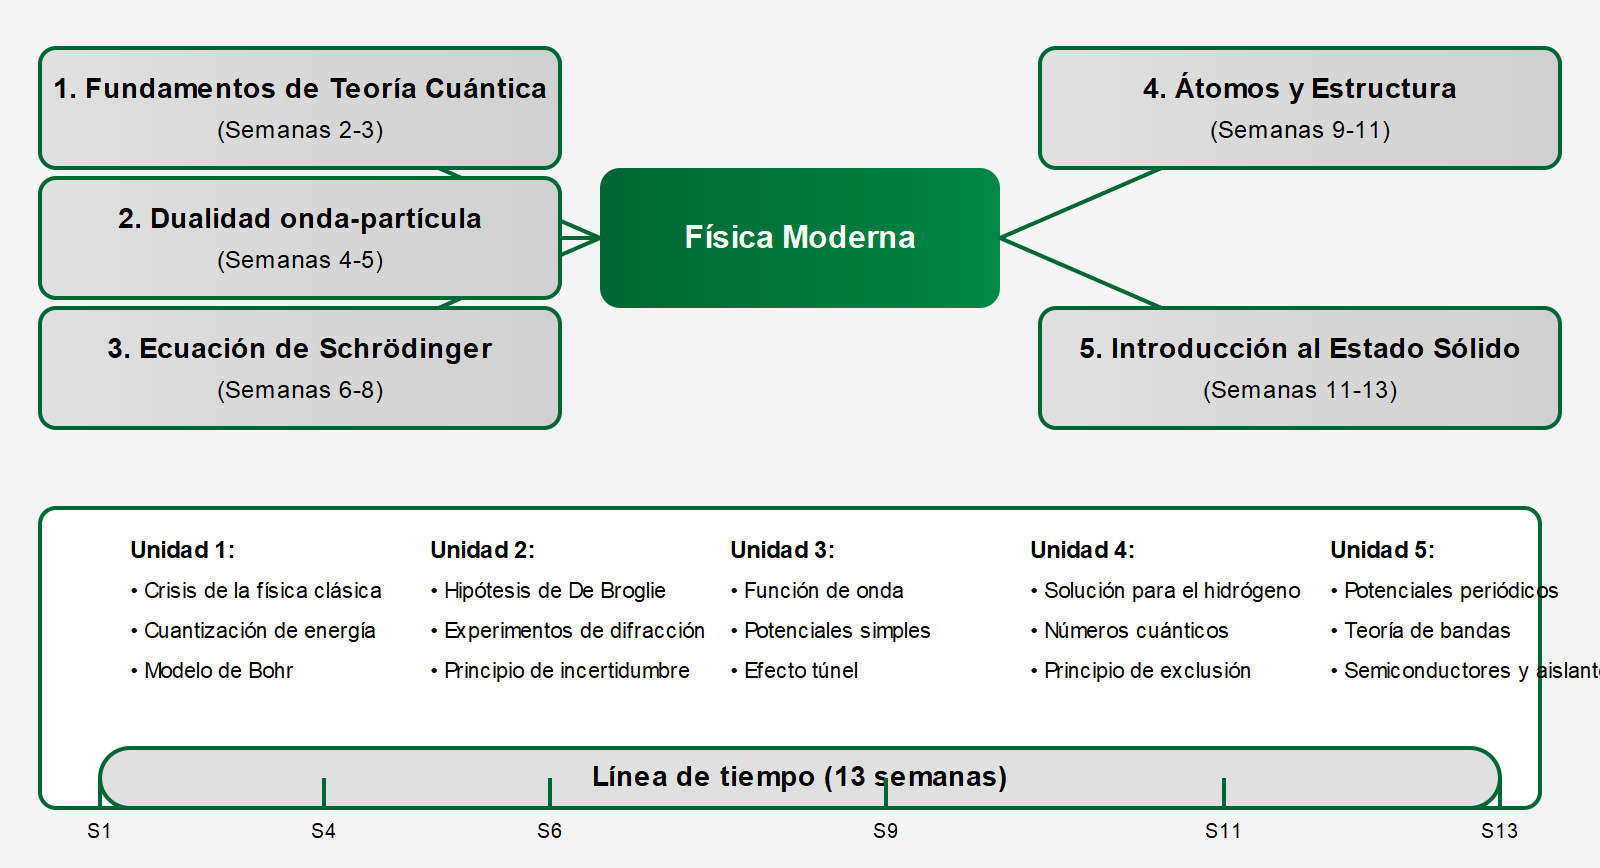
\includegraphics[width=1\linewidth]{../Imagenes/mapafisica.png}
		%\caption{The caption of the figure.}
	\end{figure}	
	
	%% TODO: You can add the note here
	\note{}	
\end{frame}

\begin{frame}
	\frametitle{Políticas Institucionales}
	\begin{enumerate}
		\item Para tener derecho a asistir a clases y evaluaciones, es requisito estar inscritos oficialmente.
		\item Utilizaremos el correo institucional como medio oficial de comunicación.
		\item El plagio está estrictamente prohibido. Cualquier trabajo que no sea de su autoría resultará en la pérdida del derecho a aprobar la evaluación correspondiente.
		\item Se requiere un mínimo de 80\% de asistencia para tener derecho a evaluación.
		\item Las entregas deben ser puntuales y cumplir con los criterios establecidos.
		\item Las inasistencias solo pueden justificarse por causas específicas como enfermedad con incapacidad o solicitud de autoridad.
	\end{enumerate}

\end{frame}	

\begin{frame}
	\frametitle{Políticas Específicas del Curso}
	
	\textbf{Aspectos Académicos:}
	
	\begin{itemize}
		\item Entrega puntual de actividades con penalización por retraso
		\item Originalidad en todos los trabajos
		\item Uso ético y declarado de herramientas de IA
	\end{itemize}

	\textbf{Uso de Tecnología:}
	
	\begin{itemize}
		\item Aprovechar simulaciones y herramientas de IA como apoyo
		\item Enfoque en comprensión conceptual, no solo en resultados
	\end{itemize}
	
\end{frame}





\begin{frame}
    \frametitle{Metodología de Enseñanza-Aprendizaje}
    
    \textbf{Sesiones Sincrónicas (en clase)}
    \begin{itemize}
        \item Exposición dialogada
        \item Resolución guiada de problemas
        \item Trabajo con simulaciones
        \item Discusión y colaboración
    \end{itemize}
    \vspace{0.3cm}
    
    \textbf{Actividades Asincrónicas (Google Classroom)}
    \begin{itemize}
        \item Resolución de problemas
        \item Uso guiado de herramientas de IA
        \item Reportes de simulación
        \item Foros de discusión
    \end{itemize}
\end{frame}

\begin{frame}
    \frametitle{Uso de Tecnología}
    
    \textbf{Simulaciones}
    \begin{itemize}
        \item PhET Interactive Simulations
        \item Otras simulaciones específicas
    \end{itemize}
    \vspace{0.3cm}
    
    \textbf{Herramientas de IA}
    \begin{itemize}
        \item Asistentes conversacionales para:
        \begin{itemize}
            \item Profundizar conceptos
            \item Obtener explicaciones alternativas
            \item Verificar pasos en resolución de problemas
            \item Buscar información complementaria
        \end{itemize}
    \end{itemize}
\end{frame}

\begin{frame}
    \frametitle{Evaluación}
    
    \textbf{Requisito de asistencia:}
    \begin{itemize}
        \item Mínimo 80\% para tener derecho a evaluación
    \end{itemize}
    \vspace{0.2cm}
    
    \textbf{Evaluación Diagnóstica (0\%)}
    \begin{itemize}
        \item Cuestionario inicial (hoy)
    \end{itemize}
    \vspace{0.2cm}
    
    \textbf{Evaluación Formativa (30\%)}
    \begin{itemize}
        \item Portafolio digital de problemas (10\%)
        \item Reportes de simulaciones (10\%)
        \item Participación y foros (5\%)
        \item Autoevaluación/coevaluación (5\%)
    \end{itemize}
    \vspace{0.2cm}
    
    \textbf{Evaluación Sumativa (70\%)}
    \begin{itemize}
        \item Evaluaciones de unidad (5 × 10\% = 50\%)
        \item Proyecto integrador final (20\%)
    \end{itemize}
\end{frame}

\begin{frame}
    \frametitle{Niveles de Desempeño}
    
    \textbf{SA (Satisfactorio)}
    \begin{itemize}
        \item Comprensión básica de principios fundamentales
        \item 80\% de actividades formativas con calidad aceptable
        \item Mínimo 70\% en evaluaciones sumativas
    \end{itemize}
    \vspace{0.2cm}
    
    \textbf{DE (Destacado)}
    \begin{itemize}
        \item Comprensión profunda de conceptos
        \item 100\% de actividades con alta calidad
        \item Mínimo 85\% en evaluaciones sumativas
    \end{itemize}
    \vspace{0.2cm}
    
    \textbf{AU (Autónomo)}
    \begin{itemize}
        \item Pensamiento crítico avanzado
        \item Soluciones originales a problemas complejos
        \item Mínimo 95\% en evaluaciones sumativas
    \end{itemize}
\end{frame}

\begin{frame}
    \frametitle{Recursos Principales}
    
    \textbf{Bibliografía Base}
    \begin{itemize}
        \item Griffiths, D. (2016). \textit{Quantum Mechanics}
        \item Eisberg, R., \& Resnick, R. \textit{Física cuántica}
        \item Serway, R. A., Moses, C. J., \& Moyer, C. A. (2005). \textit{Física moderna}
        \item Tipler, P. A. (2012). \textit{Física Moderna}
    \end{itemize}
    \vspace{0.3cm}
    
    \textbf{Recursos Digitales}
    \begin{itemize}
        \item Simulaciones PhET
        \item Classroom: código de acceso [insertar código]
        \item Repositorio de recursos digitales
    \end{itemize}
\end{frame}

\begin{frame}
    \frametitle{Políticas del Curso}
    
    \textbf{Aspecto Académico}
    \begin{itemize}
        \item Entrega puntual de actividades
        \item Originalidad en trabajos
        \item Uso ético de herramientas de IA
    \end{itemize}
    \vspace{0.3cm}
    
    \textbf{Uso de Tecnología}
    \begin{itemize}
        \item Aprovechar simulaciones y herramientas IA como apoyo
        \item Declarar uso de IA en trabajos cuando corresponda
        \item Enfoque en comprensión conceptual, no solo en resultados
    \end{itemize}
\end{frame}

\begin{frame}
    \frametitle{Políticas de Clase Institucionales}
    \begin{enumerate}
        \item Para tener derecho a asistir a clases y a la evaluación del aprendizaje correspondiente, será requisito que los alumnos estén inscritos oficialmente.
        
        \item Los alumnos contarán con correo institucional, que será el medio oficial para la comunicación y entrega de reportes, trabajos o actividades asignadas en la plataforma de Google.
        
        \item El plagio de tareas, proyectos, presentaciones, evaluaciones o prácticas, queda estrictamente prohibido. El alumno que sea sorprendido entregando resultados que no sean de su autoría, perderá derecho a aprobar la evaluación correspondiente.
    \end{enumerate}
\end{frame}

\begin{frame}
    \frametitle{Políticas de Clase Institucionales}
    \begin{enumerate}\setcounter{enumi}{3}
        \item El alumno tendrá derecho a la evaluación del aprendizaje siempre y cuando cumpla con las actividades encomendadas y entregue en tiempo y forma los productos de aprendizaje señalados.
        
        \item La puntualidad y asistencia, así como las actitudes y valores son criterios para evaluar el saber ser y aprobar la unidad en la fase ordinaria. El porcentaje mínimo de asistencia será del 80\% del total de horas de la unidad.
        
        \item El estudiante podrá justificar alguna inasistencia solamente en caso de incapacidad por enfermedad o a solicitud de alguna autoridad educativa, familiar o empresa debido a alguna situación especial.
    \end{enumerate}
\end{frame}

\begin{frame}
    \frametitle{¿Qué esperar del curso?}
    
    \textbf{Semana 1}
    \begin{itemize}
        \item Hoy: Presentación y diagnóstico
        \item Próxima sesión: Repaso de conceptos de electromagnetismo clásico
    \end{itemize}
    \vspace{0.2cm}
    
    \textbf{Semanas 2-13}
    \begin{itemize}
        \item Desarrollo de las unidades temáticas
        \item Actividades prácticas y simulaciones
        \item Evaluaciones programadas
    \end{itemize}
    \vspace{0.2cm}
    
    \textbf{A lo largo del curso}
    \begin{itemize}
        \item Conexión entre teoría cuántica y nanotecnología
        \item Construcción progresiva de competencias
        \item Aplicación práctica de conocimientos
    \end{itemize}
\end{frame}

\begin{frame}
    \frametitle{Evaluación Diagnóstica}
    
    A continuación realizaremos:
    \begin{enumerate}
        \item Presentación breve de cada estudiante
        \item Expectativas sobre el curso
        \item Cuestionario diagnóstico (Google Forms)
        \item Discusión sobre uso ético de IA como herramienta de aprendizaje
    \end{enumerate}
\end{frame}

\begin{frame}
    \frametitle{¡Comencemos!}
    
    \textbf{Contacto:}
    \begin{itemize}
        \item Correo electrónico: [insertar correo]
        \item Horario de consulta: [insertar horario]
        \item Classroom: [insertar enlace]
    \end{itemize}
    \vspace{0.8cm}
    
    \begin{center}
        \Large ¿Preguntas?
    \end{center}
\end{frame}

\end{document}